\documentclass{article}
\usepackage{tikz}

\newcommand{\DrawParallelLines}[2]{ % #1 = y-offset, #2 = rotation
    \begin{scope}[rotate=#2]
        \draw[thick, blue] (-3,#1) -- (3,#1);
        \draw[thick, blue] (-4,#1+1) -- (4,#1+1);
    \end{scope}
}

\begin{document}

\begin{center}
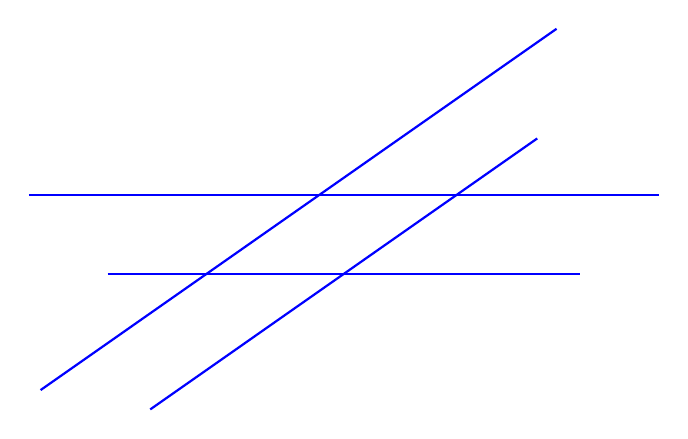
\begin{tikzpicture}

    % Original lines (before rotation)
    \DrawParallelLines{0}{0}  % No rotation (Green)
    
    % Rotated lines (35 degrees)
    \DrawParallelLines{0}{35}  % Rotated by 35 degrees

\end{tikzpicture}
\end{center}

\end{document}
